\newpage
\section{Formal description of data structure and metadata}
\label{sec:metadata}

\subsection{What do rows of the data matrix contain}

Each row in the dataset represents a \textbf{unique ifood customer}. The dataset includes
their \textbf{demographic profile} (education level, marital status, yearly income,
number of children and teenagers), \textbf{relationship indicators} (recency in days
since last purchase, complaint history, and campaign responses), and \textbf{purchase
behavior} over the last two years. Purchases are detailed by \textit{product category}
(wine, fruits, meat, fish, sweets, gold) and \textit{sales channel} (web, catalog,
store, discounted purchases, and website visits).

Two dataset versions were used throughout this study:
\begin{itemize}
    \item \texttt{ifood\_base}: the original raw dataset (\(2{,}240 \times 29\)).
    \item \texttt{ifood\_enriched}: the preprocessed and feature-engineered dataset (\(2{,}031 \times 40\)).
\end{itemize}

The enriched version introduces engineered variables (e.g., \textit{Age}, \textit{TotalExp},
\textit{TotalPurchases}, \textit{AvgSpendPerPurchase}, \textit{PreferredChannel},
\textit{CustomerSegment}), standardized naming conventions, and cleaned variable
types, while maintaining the same observational unit: the individual customer.

\vspace{0.5em}

\subsection{Metadata Table}

The complete metadata dictionary was generated through the script
\texttt{metadata\_ifood.Rmd} and exported as visual tables. The following figures
(\autoref{fig:metadata1} and \autoref{fig:metadata2}) present the official metadata
captured from the base dataset, including data type, description, and possible
values.

\begin{figure}[H]
    \centering
    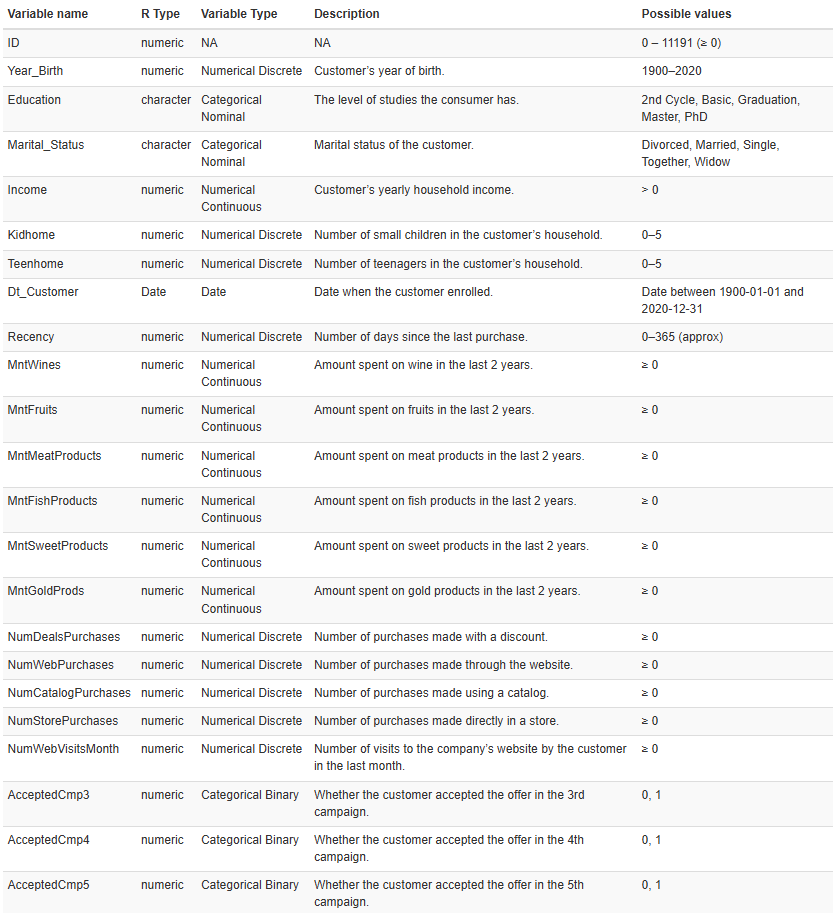
\includegraphics[width=0.95\textwidth]{Imatges/metadata6.png}
    \caption{Automatically generated metadata dictionary (part 1) from \texttt{metadata\_ifood.Rmd}.}
    \label{fig:metadata1}
\end{figure}

\begin{figure}[H]
    \centering
    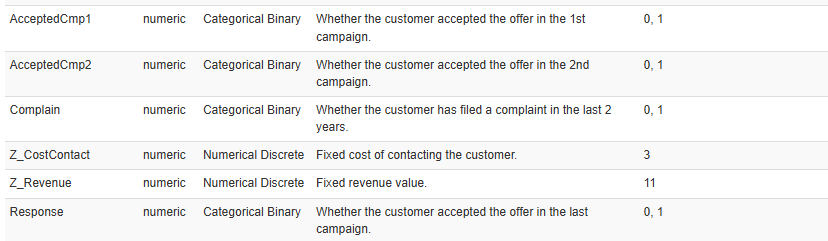
\includegraphics[width=0.95\textwidth]{Imatges/metadata7.png}
    \caption{Automatically generated metadata dictionary (part 2) from \texttt{metadata\_ifood.Rmd}.}
    \label{fig:metadata2}
\end{figure}

\noindent
\textbf{Data quality summary:} In \texttt{ifood\_base}, only \textit{Income} contained missing values
($\approx 1.07\%$). In \texttt{ifood\_enriched}, all variables used for analysis were
fully complete after imputation and cleaning.

\vspace{0.5em}

\subsection{Final scope and inclusion/exclusion criteria}

\textbf{Analytical scope.}
The final analytical dataset (\texttt{ifood\_enriched}) contains \(2{,}031\) rows and \(40\)
variables, corresponding to a reduction of 209 records (−9.33\%) from the raw
dataset after cleaning and standardization.

\textbf{Row-level inclusion/exclusion:}
\begin{itemize}
    \item \textit{Included:} customers with valid demographic, behavioral, and response information.
    \item \textit{Excluded:}
    \begin{itemize}
        \item Records with missing or inconsistent key variables (e.g., invalid income or age).
        \item Extreme or illogical values identified during preprocessing (e.g., negative totals).
        \item Observations removed during data integrity validation or outlier filtering.
    \end{itemize}
\end{itemize}

\textbf{Column-level inclusion/exclusion:}
\begin{itemize}
    \item \textit{Removed:} identifiers and administrative variables (\texttt{ID}, \texttt{Dt\_Customer},
    \texttt{Z\_CostContact}, \texttt{Z\_Revenue}).
    \item \textit{Renamed:}
    \begin{itemize}
        \item \texttt{Marital\_Status} $\rightarrow$ \texttt{MaritalSts}
        \item \texttt{Mnt*} $\rightarrow$ \texttt{*Exp} (e.g., \texttt{MntWines} $\rightarrow$ \texttt{WineExp})
        \item \texttt{Num*Purchases} $\rightarrow$ \texttt{*Purc} (e.g., \texttt{NumCatalogPurchases} $\rightarrow$ \texttt{CatalogPurc})
    \end{itemize}
    \item \textit{Added engineered features:} \texttt{Age}, \texttt{TotalExp}, \texttt{TotalPurchases},
    \texttt{AvgSpendPerPurchase}, \texttt{TotAccCmp}, \texttt{CampaignAcceptanceRate},
    \texttt{PreferredProductCategory}, \texttt{PreferredChannel}, \texttt{HasChildren},
    \texttt{IncomeSegment}, \texttt{CustomerSegment}, \texttt{PropensityScore}, and \texttt{EngagementIndex}.
\end{itemize}

\noindent
\textbf{Final dataset:} 2,031 customers $\times$ 40 variables with clean,
well-typed data and engineered features that capture \textit{purchase intensity},
\textit{channel/product preferences}, and \textit{marketing responsiveness},
ready for the subsequent data mining and modeling phases.


% ============================================================
% 6. COMPLETE DATA MINING PROCESS PERFORMED
% ============================================================
\newpage
\section{Complete Data Mining process performed}

The complete Data Mining workflow followed the standard \textbf{CRISP--DM}
(Cross‐Industry Standard Process for Data Mining) methodology, adapted to the
context of customer segmentation and campaign‐response analysis.  
The process was entirely documented and implemented through R and R Markdown scripts
(\texttt{metadata\_ifood.Rmd}, \texttt{Preprocessing.R}) and reproducible
CSV outputs (\texttt{ifood\_base.csv}, \texttt{ifood\_enriched.csv}).

\subsection{Overview of the process}

\begin{figure}[H]
    \centering
    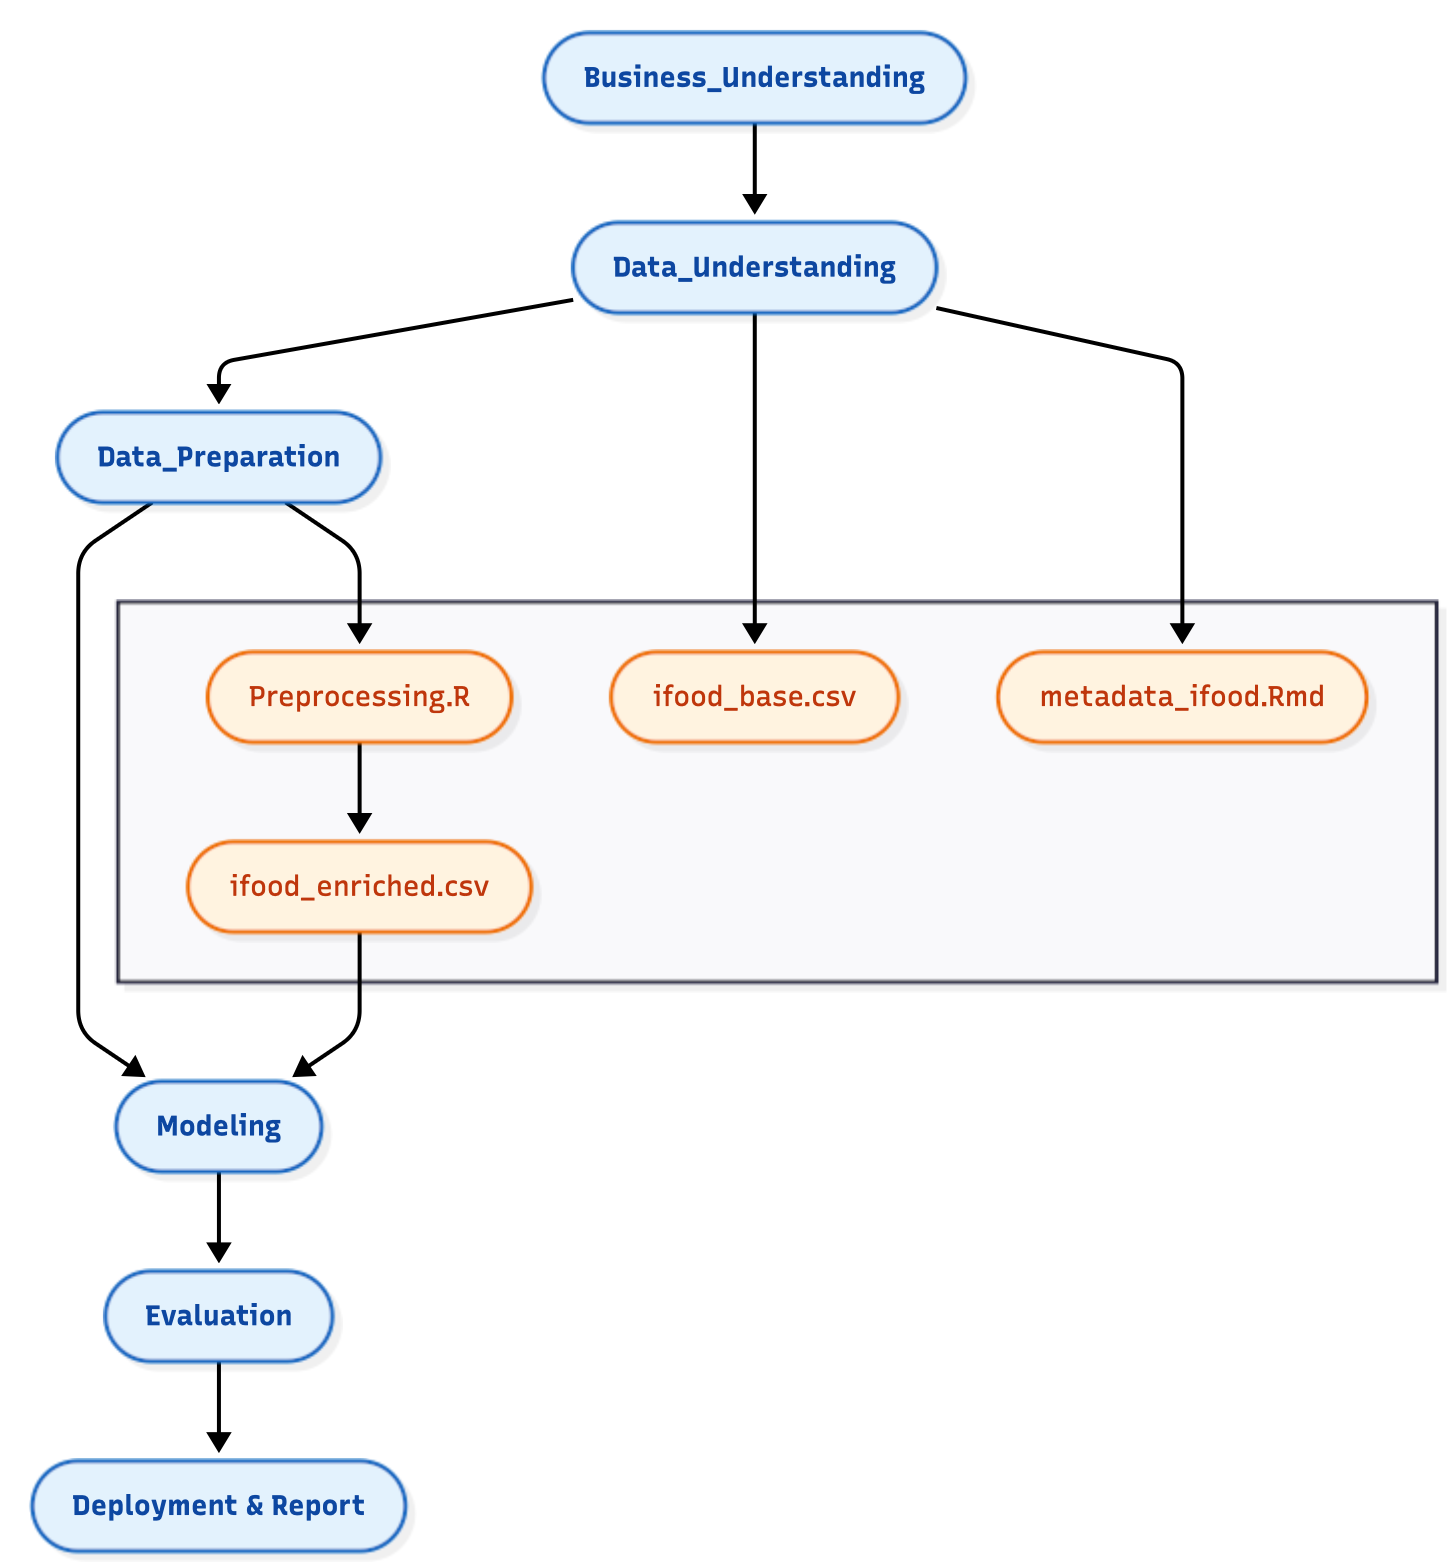
\includegraphics[width=0.9\textwidth]{Imatges/workflow_datamining.png}
    \caption{Simplified CRISP--DM workflow applied to the ifood project.}
    \label{fig:workflow_dm}
\end{figure}

\subsubsection*{Complementary workflow description}

Figure~\ref{fig:workflow_dm} illustrates the main stages and data flow of the study.  
Each phase of the CRISP--DM cycle is directly connected to the corresponding implementation files within the repository:

\begin{itemize}[leftmargin=1.2cm]
    \item \textbf{Data sources:} process starts from the raw dataset \texttt{ifood\_base.csv}.
    \item \textbf{Metadata generation:} script \texttt{metadata\_ifood.Rmd} performs variable inspection and produces the metadata in Section~\ref{sec:metadata}.
    \item \textbf{Preprocessing:} handled in \texttt{Preprocessing.R}, applying cleaning, imputation, renaming, and feature engineering to create \texttt{ifood\_enriched.csv}.
    \item \textbf{Modeling inputs:} the enriched dataset supports clustering and classification analyses.
    \item \textbf{Outputs:} final datasets, figures, and reports are exported as reproducible files.
\end{itemize}

\subsection{Detailed description of the process}

\begin{enumerate}
    \item \textbf{Business understanding:} define the analytical goal --- identify customer patterns and features explaining campaign response.
    \item \textbf{Data understanding:} explore \texttt{ifood\_base.csv} for types, ranges, and completeness using \texttt{metadata\_ifood.Rmd}.
    \item \textbf{Data preparation:} clean data, impute missing \textit{Income}, rename columns, encode categorical variables, engineer features (\textit{Age}, \textit{TotalExp}, \textit{AvgSpendPerPurchase}, etc.), and scale numeric variables for modeling.
    \item \textbf{Modeling:} apply unsupervised (K‐means, hierarchical clustering) and supervised (logistic regression, decision tree) models on \texttt{ifood\_enriched.csv}.
    \item \textbf{Evaluation:} assess clustering via silhouette width/inertia and classification via accuracy, recall, AUC; visualize results.
    \item \textbf{Deployment and reporting:} compile reproducible reports and final datasets (\texttt{ifood\_enriched.csv}) for future use.
\end{enumerate}

\subsection{Summary}

This end‐to‐end process guarantees \textbf{traceability, reproducibility, and
interpretability}. Every transformation is documented in the preprocessing scripts,
and the resulting dataset aligns with the metadata in Section~\ref{sec:metadata}.


% ============================================================
% 7. DETAILED DESCRIPTION OF PREPROCESSING AND DATA PREPARATION
% ============================================================
\newpage
\section{Detailed description of Preprocessing and Data Preparation}

This section provides an in‐depth description of the preprocessing pipeline
implemented in \texttt{Preprocessing.R}, which transforms
\texttt{ifood\_base.csv} into the final analytical matrix
\texttt{ifood\_enriched.csv}.  
Transformations were applied based on the exploratory results of
\texttt{metadata\_ifood.Rmd}, ensuring full consistency with Section~\ref{sec:metadata}.

\subsection{Data cleaning and integrity checks}

\begin{itemize}[leftmargin=1.2cm]
    \item \textbf{Duplicates and invalid records:} removed, reducing the dataset
    from 2,240 to 2,031 observations (−9.33\%).
    \item \textbf{Consistency validation:} checked numerical ranges (e.g.,
    \textit{Recency}, \textit{Income}, \textit{Age}) and removed outliers.
    \item \textbf{Missing values:} only \textit{Income} had NA values
    ($\approx$1.07\%); imputed using the median.
\end{itemize}

\subsection{Variable transformation and standardization}

\begin{itemize}[leftmargin=1.2cm]
    \item \textbf{Renaming:} standardized names
    (\texttt{MntWines}→\texttt{WineExp}, \texttt{NumWebPurchases}→\texttt{WebPurc},
    \texttt{Marital\_Status}→\texttt{MaritalSts}).
    \item \textbf{Type correction:} categorical and binary variables cast to proper types.
    \item \textbf{Scaling:} expenditure and frequency variables standardized (z‐score)
    for algorithms sensitive to magnitude differences.
\end{itemize}

\subsection{Encoding of categorical variables}

\begin{itemize}[leftmargin=1.2cm]
    \item \textbf{Binary encoding:} \textit{AccCmp1–AccCmp5}, \textit{Complain},
    \textit{Response}, \textit{HasChildren}.
    \item \textbf{One‐hot encoding:} \textit{MaritalSts}, \textit{Education}.
    \item \textbf{Ordinal encoding:} \textit{IncomeSegment} (Low–High),
    \textit{CustomerSegment} (1–3).
\end{itemize}

\subsection{Feature engineering}

\begin{itemize}[leftmargin=1.2cm]
    \item \textbf{Age:} derived from birth year.
    \item \textbf{TotalExp:} sum of all expenditures (wine, fruits, meat, fish, sweets, gold).
    \item \textbf{TotalPurchases:} total number of purchases across channels.
    \item \textbf{AvgSpendPerPurchase:} ratio of \textit{TotalExp}/\textit{TotalPurchases}.
    \item \textbf{HasChildren:} derived from \textit{Kidhome} or \textit{Teenhome}.
    \item \textbf{PreferredChannel/Product:} channel or category with highest frequency.
    \item \textbf{CustomerTenure (CustDays):} estimated relationship duration.
    \item \textbf{TotAccCmp, CampaignAcceptanceRate:} aggregate campaign engagement.
    \item \textbf{IncomeSegment, CustomerSegment:} segmentations by quantile thresholds.
    \item \textbf{PropensityScore, EngagementIndex:} composite behavioral indices.
\end{itemize}

\subsection{Feature selection and validation}

\begin{itemize}[leftmargin=1.2cm]
    \item Removed variables with $>$30\% missing data or redundancy.
    \item Checked correlations ($|r|>0.95$) to avoid multicollinearity.
    \item Retained 40 variables relevant for clustering and prediction.
\end{itemize}

\subsection{Resulting dataset and export}

The final matrix \texttt{ifood\_enriched.csv} contains 2,031 fully cleaned,
encoded, and standardized observations and variables.

\subsection{Summary}

The preprocessing workflow ensured \textbf{data consistency, interpretability, and reproducibility}.
All transformations were documented within the R Markdown environment,
providing full traceability from raw data to enriched dataset.  
This structure enables robust analyses for customer segmentation and campaign
targeting, concluding the data preparation phase of the project.